\documentclass[12pt]{article}
\usepackage{graphicx}
\usepackage{graphics}
\usepackage{url}

\title{MoViSign: A novel authentication mechanism using mobile virtual signatures}
\author{Nikhil Handigol, Te-Yuan Huang, Gene Chi Liu}
\date{}

\begin{document}
\maketitle


\section{Introduction}

Signatures are a popular means of authentication. They, ideally, are unique to a person and, therefore, hard to copy. Two common types of signatures are traditional ``pen-on-paper'' signatures and electronic signatures. Electronic signatures are done on a custom-built electronic board using a stylus. The electronic board records information such as pressure, acceleration, and angle of the stylus in addition to the standard signature ``image''. This information is used by a signature recognition system to differentiate authentic signatures from fraudulent ones. Both types of signatures have their drawbacks. While traditional ``pen-on-paper'' signatures are prone to forgery by expert humans, electronic signatures require a special electronic board to record the signature.

In this project, we design and implement a novel mechanism of authentication, called mobile virtual signature, using mobile phones. Modern mobile phones such as the Apple iPhone and the Google G-phone are equipped with multiple sensors including accelerometers, orientation sensors, temperature sensors, proximity sensors, and multi-touch sensors. In our authentication mechanism, a person authenticates by signing ``in the air'' with the phone. The sensors on the phone, primarily the accelerometer and the orientation sensor, continuously record various parameters such as position, acceleration and angle. This information is then used by a Machine Learning program running on the mobile phone to recognize the signature.

The authentication mechanism has several advantages. First, just like the traditional signatures, mobile virtual signatures stay unique to each person and can be changed if necessary. Second, it makes forgery hard as the signature is made ``in the air'' and without producing any tangible output to copy from. Third, it is hard to map the information collected by the accelerometers back to the actual physical movement that produced the signature. Finally, the mechanism uses popular mobile phones, and hence can be deployed on a large scale without additional cost.

We have developed a prototype of the system on the Google G-phone. The G-phone runs the open source Android operating system which allows for easy development of new applications and reuse of components built by other developers.

\section{System Design}

We have implemented a Java application on Android to collect values from accelerometer and orientation sensors as our training set and run an SVM-based learning algorithm to classify authentic and non-authentic signatures.

The values from the accelerometer sensor are defined in the accelerometer reference~\cite{accelerometer}. We record acceleration in the X, Y and Z axes, whose positive directions are toward the right side, top, and front of the device respectively.

The values from the orientation sensor are defined in the orientation sensor reference~\cite{orientation}.
We record three values from the orientation sensor~\cite{orient1}:

\begin{figure}[ht]
\begin{minipage}[b]{0.3\textwidth}
\centering
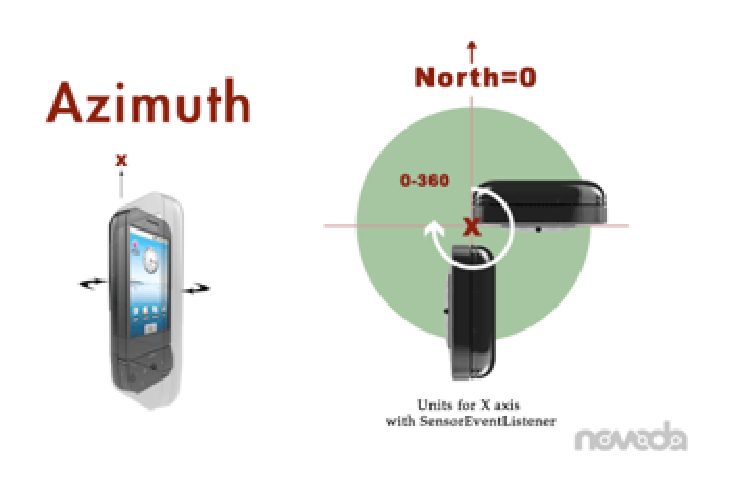
\includegraphics[width=\textwidth]{azimuth}
\caption{Azimuth}
\label{fig:azimuth}
\end{minipage}
\begin{minipage}[b]{0.3\textwidth}
\centering
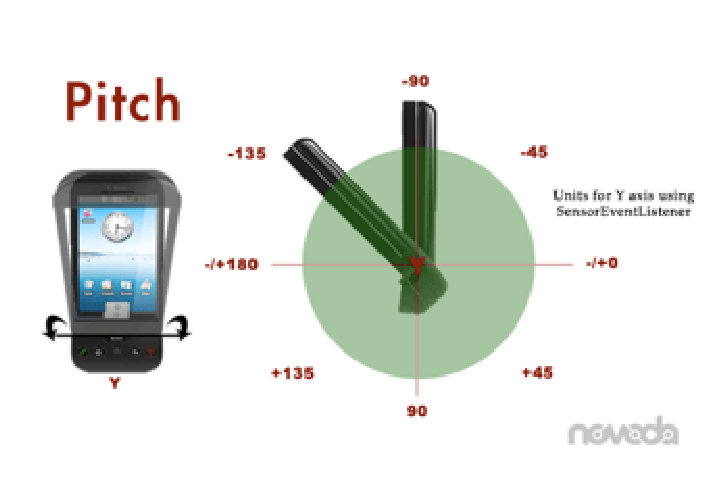
\includegraphics[width=\textwidth]{pitch}
\caption{Pitch}
\label{fig:pitch}
\end{minipage}
\begin{minipage}[b]{0.3\textwidth}
\centering
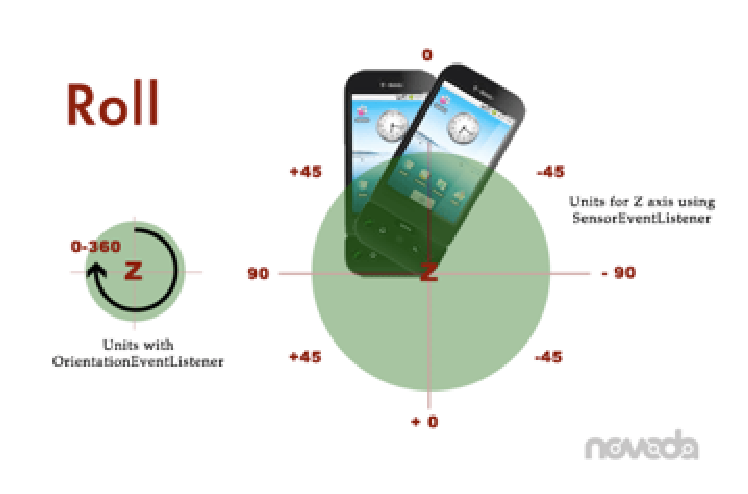
\includegraphics[width=\textwidth]{roll}
\caption{Roll}
\label{fig:roll}
\end{minipage}
\end{figure}

\begin{itemize}
\item Azimuth(Figure~\ref{fig:azimuth}) - the angle in current reference to magnetic north, ranges between [0. 360]. 
\item Pitch(Figure~\ref{fig:pitch}) - the degree to which the device is tilted forwards or backwards, ranges between [-180, 180].
\item Roll(Figure~\ref{fig:roll}) - the rotation of the device in relation to the bottom left hand corner of the screen, ranges between [-90, 90].
\end{itemize}

Using this application, the user can create input samples and label them as ``authentic'' or ``non-authentic''. The application logs each input sample into a file, which is then used by the machine learning algorithm to train/test the authenticity of the input signature.

\section{User Interface}

\begin{figure}[ht]
\label{fig:gui}
\begin{minipage}[b]{0.3\textwidth}
\centering
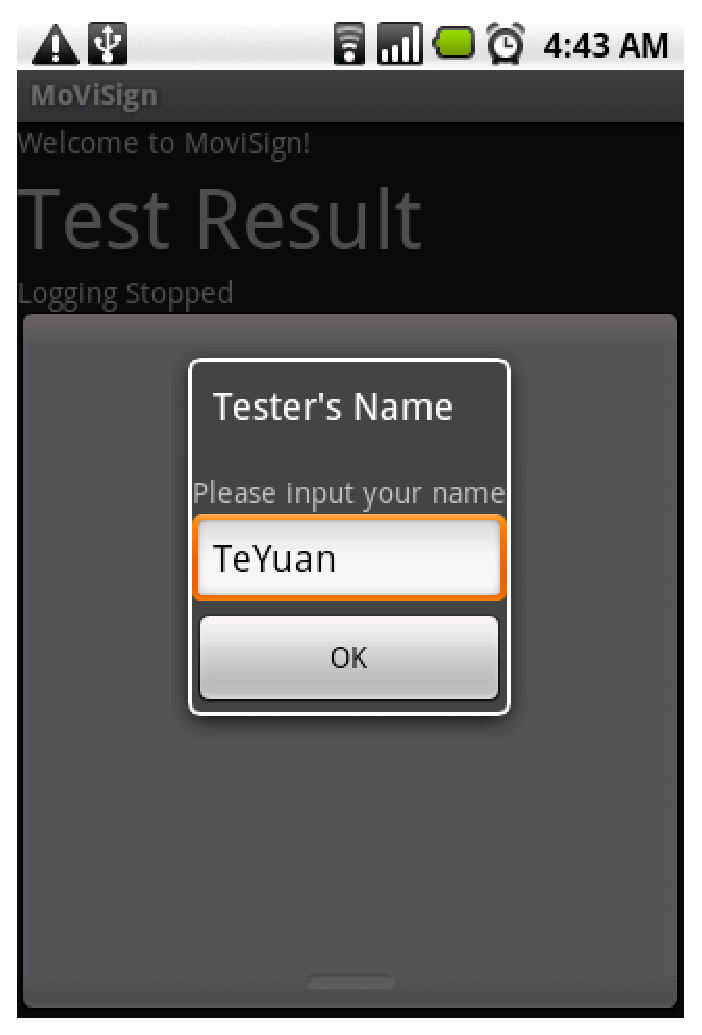
\includegraphics[width=\textwidth]{name}
\caption{Entering user name.}
\label{fig:name}
\end{minipage}
\begin{minipage}[b]{0.3\textwidth}
\centering
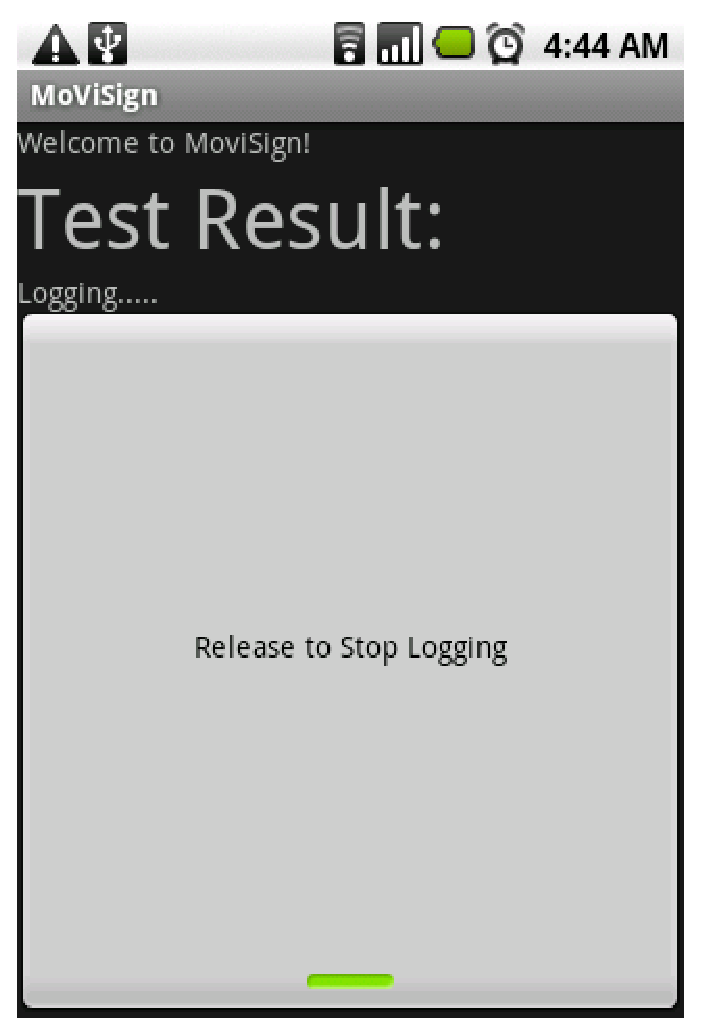
\includegraphics[width=\textwidth]{logging}
\caption{Data logging.}
\label{fig:logging}
\end{minipage}
\begin{minipage}[b]{0.3\textwidth}
\centering
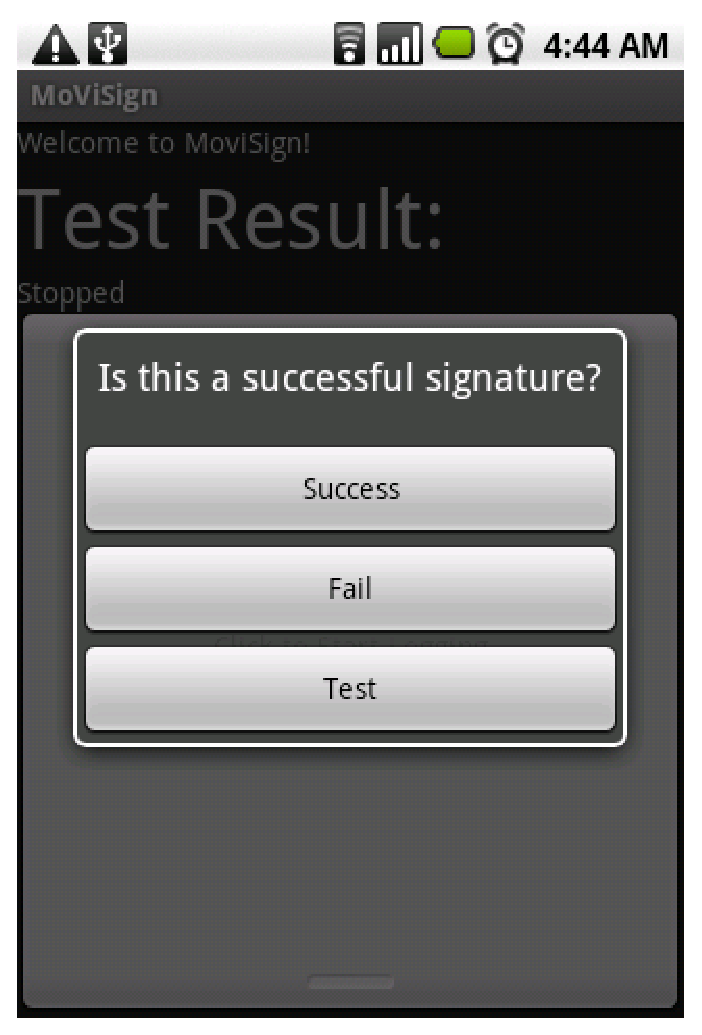
\includegraphics[width=\textwidth]{checkbox}
\caption{Training/testing the data}
\label{fig:checkbox}
\end{minipage}
\end{figure}

Figures~\ref{fig:name},~\ref{fig:logging}, and~\ref{fig:checkbox} show the graphical user interface (GUI) of the MoViSign system. The user begins by giving her name as the input after which she will be presented with a ``log'' button. The user then signs her signature while holding the ``log'' button down, and then releases the button. After the signature logging, the user is presented with 3 options:
\begin{itemize}
\item Success - Use the logged data as an authentic signature to train the system.
\item Fail - Use the logged data as an non-authentic signature to train the system.
\item Test - Test the authenticity of the signature based on the training data.
\end{itemize}

\section{Training and Evaluation}

\textbf{Test Data}:
We generated about 400 signatures, including two of our group members' signatures. Each of the two signed for about 100 times as positive training data, and about 200 irrelevant patterns as negative training data.

\textbf{Feature Extraction}:
For each signature, we log the output of the accelerometer and orientation sensor and store them in increasing time order based on timestamp. We then divide the log data evenly into $s$ segments (for $s = 2,4,8,16,32$.). For each segment, compute the mean of accelerometer readings ( in x, y, z directions, respectively) and orientation sensor (in aziroth, pitch, roll, respectively). We then use these six mean values as features for that particular data segment. Thus, we have $6*s$ features for each signature.

\textbf{Training}:
We use SVM with linear kernel and L1 soft margin. Our SVM is implemented using CVX, a convex optimization problem solver built on MATLAB (http://www.stanford.edu/~boyd/cvx/). We use C = 100 for the L1 soft margin. We use a very large C here so that the alpha values will not be affected by L1 soft margin constraint in most cases.

\textbf{Evaluation}:
Our first attempt was to use Leave-one-out cross validation. As it took too much time to train and evaluate on every single test data, we also tried K-fold cross validation for K = 20 on larger data sets.

\textbf{Discussion}:
(relationships between number of segments and error rate)
(the difference between leave-one-out and 20-fold cross validation)

\section{Related Work}

Our authentication mechanism falls in the category of online signature recognition. Previous work on online signature recognition~\cite{zanuy:2006} uses position(x, y), pressure, and orientation of the stylus on the electronic board as the input features. The system stores preprocessed genuine signatures captured from each user. It then uses dynamic time warping and HMM models to compute the similarity between the new input signature and the stored genuine signatures.

MoViSign differs from the previous work in terms of both the feature-set and the classification mechanism. MoViSign uses 3-D position, and orientation based on signatures generated by hand-gestures using mobile devices. It then uses supervised machine learning algorithm to classify signatures as aunthentic and fake ones.
 
\section{Conclusion}

Mobile virtual signature is a novel and potentially useful application of mobile phones. In this project, we designed and implemented the system using a simple SVM-based machine learning algorithm. Our results show that the algorithm does a good job of classifying signatures, with very low error rates.

\bibliographystyle{plain}
\bibliography{ref}	

\end{document}
